In \scnref{scn:techs} we showed how Dippy works in practice by making customisations to the solver framework for an example problem.
We will use the Wedding Planner problem from the PuLP documentation \cite{pulp} to compare Dippy to two leading solvers that utilise branch-and-cut: the open-source CBC and the commercial Gurobi.
This particular problem is useful for comparing performance because it has a natural column generation formulation and can be scaled-up in a simple way, unlike the Facility Location problem which is strongly dependent on the specific instance being tested.

The Wedding Planner problem is as follows: given a list of wedding attendees, a wedding planner must come up with a seating plan to minimise the unhappiness of all of the guests.
The unhappiness of guest is defined as their maximum unhappiness at being seated with each of the other guests at their table, making it a pairwise function.
The unhappiness of a table is the maximum unhappiness of all the guests at the table.
All guests must be seated and there is a limited number of seats at each table.

This is a set partitioning problem, as the set of guests $G$ must be partitioned into multiple subsets, with the members of each subset seated at the same table.
The cardinality of the subsets is determined by the number of seats at a table and the unhappiness of a table can be determined by the subset.
The \ac{MILP} formulation is:
\[
\begin{array}{rrl}
& x_{gt} &= \begin{cases} 1 & \text{if guest $g$ sits at table $t$} \\
 0 & \text{otherwise} \end{cases} \\
& u_t &= \text{unhappiness of table $t$} \\
& S &= \text{number of seats at a table} \\
& U(g, h) &= \text{unhappiness of guests $g$ and $h$ if they are seated at the same table}
\end{array}
\]\[
\begin{array}{rrl}
\min & \displaystyle \sum_{t \in T} u_t & \text{(total unhappiness of the tables)} \\
& \displaystyle \sum_{g \in G} x_{gt} &\leq S, t \in T \\
& \displaystyle \sum_{t \in T} x_{gt} &=1, g \in G \\
& u_t &\geq U(g, h) (x_{gt} + x_{ht} - 1), t \in T, g < h \in G
\end{array}
\]

Since \ac{DIP}, and thus Dippy, doesn't require a problem to be explicitly formulated as a Dantzig-Wolfe decomposition, a change from \ac{DIP} to CBC is trivial.
The only differences are that:
\begin{enumerate}
\item A \lstinline{LpProblem} is created instead of a \lstinline{DipProblem};
\item No \lstinline{.relaxation} statements are used;
\item The \lstinline{LpProblem.solve} method uses CBC to solve the problem.
\end{enumerate}
To see if CBC and Gurobi would perform well with a column-based approach, we also formulated a problem equivalent to the restricted master problem from the branch-price-and-cut approach and generated and added all possible columns before the solving the \ac{MILP}.
Finally we used to Dippy to develop a customised solver and initial variable generation function for the branch-price-and-cut formulation in \ac{DIP}.
In total, six approaches were tested on problem instances of increasing size:
\begin{enumerate}
\item CBC called from PuLP;
\item CBC called from PuLP using a columnwise formulation and generating all columns a priori;
\item Gurobi called from PuLP;
\item Gurobi called from PuLP using a columnwise formulation and generating all columns a priori;
\item \ac{DIP} called from Dippy using branch-price-and-cut without customisation;
\item \ac{DIP} called from Dippy using customised branching, cuts and column generation callback functions.
\end{enumerate}

In \Tabref{tab:wed_exp} and \Figref{fig:compare} we see that\footnote{All tests were run using Python 2.7.1 on a Dell XPS1530 laptop with an Intel Core~2~Duo CPU T9500@2.60GHz and 4~GB of RAM. We used CBC version~2.30.00, Gurobi version~4.5.1, and Dippy version~1.0.10.}:
\begin{itemize}
\item Gurobi is fastest for small problems;
\item The symmetry present in the problem means the solution time of CBC and Gurobi for the original problem deteriorate quickly;
\item The time taken to solve the columnwise formulation also deteriorates, but at a lesser rate than when using CBC or Gurobi on the original problem;
\item Both \ac{DIP} and customised \ac{DIP} solution times grow at a lesser rate than any of the CBC/Gurobi approaches;
\item For large problems, \ac{DIP} becomes the preferred approach.
\end{itemize}

The main motivation for the development of Dippy was to alleviate obstacles to experimentation with and customisation of advanced \ac{MILP} frameworks.
These obstacles arose from an inability to use the description of a problem in a high-level modelling languag integrated with the callback functions in leading solvers.
This is mitigated with Dippy by using the Python-based modelling language PuLP to describe the problem and then exploiting Python's variable scoping rules to implement the callback functions.

Using the Capacitated Facility Location problem we have shown that Dippy is relatively simple to experiment with and customise, enabling the user to quickly and easily test many approaches for a particular problem, including combinations of approaches.
In practice Dippy has been used successfully to enable final year undergraduate students to experiment with advanced branching, cut generation, column generation and root/node heuristics.
%Given the demonstrated ease of the implementation of advanced \ac{MILP} techniques and the flexibility of a high-level mathematical modelling language, the above evidence that Dippy can be highly competitive solver for problems in which column generation is the preferred approach suggests that Dippy is effective as more than just an experimental ``toy'' or educational tool.
The Wedding Planner problem shows that Dippy can be a highly competitive solver for problems in which column generation is the preferred approach.
Given the demonstrated ease of the implementation of advanced \ac{MILP} techniques and the flexibility of a high-level mathematical modelling language, this suggests that Dippy is effective as more than just an experimental ``toy'' or educational tool.
It enables users to concentrate on furthering Operations Research knowledge and solving hard problems instead of spending time worrying about implementation details.
Dippy breaks down the barriers to experimentation with advanced \ac{MILP} approaches for both practitioners and researchers.


\begin{table}[htp]
\begin{minipage}[l]{\textwidth}
\begin{small}
\begin{tabular}{|l@{\,}|c@{\ }|c@{\ }c@{\ }|c@{\ }|c@{\ }c@{\ }|c@{\ }c@{\,}|}
\hline
\textbf{\# guests} & \multicolumn{8}{|c|}{\textbf{Time (s)}} \\
                   & CBC & \multicolumn{2}{c|}{CBC \& columns} & Gurobi & \multicolumn{2}{c|}{Gurobi \& columns} & \ac{DIP} & Customised \\
                   &     & gen vars & solve                    &        & gen vars & solve                       &          & \ac{DIP}   \\ 
\hline 
 6 &  0.07 & 0.01 &   0.06 &   0.04 & 0.01 &   0.05 &   0.90 &  0.33 \\
 7 &  0.07 & 0.01 &   0.12 &   0.04 & 0.01 &   0.11 &   1.77 &  0.57 \\
 8 &  0.90 & 0.01 &   0.27 &   0.07 & 0.01 &   0.25 &   4.78 &  0.57 \\
 9 &  2.54 & 0.01 &   0.57 &   0.09 & 0.01 &   0.55 &   2.11 &  0.78 \\
10 &  3.83 & 0.01 &   1.23 &   0.13 & 0.01 &   1.15 &   5.60 &  0.94 \\
11 &  6.48 & 0.01 &   2.46 &   0.14 & 0.01 &   2.36 &   8.62 &  0.91 \\
12 & 26.73 & 0.01 &   4.64 &   0.34 & 0.01 &   4.55 &  25.17 &  2.80 \\
13 & 53.18 & 0.01 &   8.57 &   0.39 & 0.01 &   8.28 &  14.86 &  1.40 \\
14 & 70.51 & 0.01 &  15.27 &   0.38 & 0.01 &  14.65 &  20.09 &  2.66 \\
15 & 97.79 & 0.01 &  26.26 &   0.47 & 0.01 &  25.07 &  33.52 &  1.59 \\
16 &$>$1000& 0.01 &  43.86 &  68.08 & 0.01 &  42.11 &  26.73 &  2.09 \\
17 &    -- & 0.01 &  72.07 &  79.71 & 0.01 &  68.87 &  50.48 &  3.92 \\
18 &    -- & 0.01 & 115.64 &  96.03 & 0.01 & 110.52 &  40.80 &  4.67 \\
19 &    -- & 0.01 & 181.39 & 113.01 & 0.01 & 173.13 &  78.20 &  2.64 \\
20 &    -- & 0.02 & 283.16 &$>$6000 & 0.01 & 270.08 &  61.86 &  5.31 \\
21 &    -- & 0.02 & 434.60 &     -- & 0.02 & 418.04 &  77.66 &  4.23 \\
22 &    -- & 0.02 & 664.87 &     -- & 0.02 & 639.04 & 134.76 &  4.63 \\
23 &    -- &   -- &$>$1000 &     -- &   -- &$>$1000 & 149.82 &  9.16 \\
24 &    -- &   -- &     -- &     -- &   -- &     -- & 110.24 &  6.51 \\
25 &    -- &   -- &     -- &     -- &   -- &     -- & 202.59 &  8.80 \\
26 &    -- &   -- &     -- &     -- &   -- &     -- & 185.21 & 18.47 \\
\hline
\end{tabular}
\end{small}
\end{minipage}
\caption{Experiments for the Wedding Planner Problem} \label{tab:wed_exp}
\end{table}

\begin{figure}[htp]
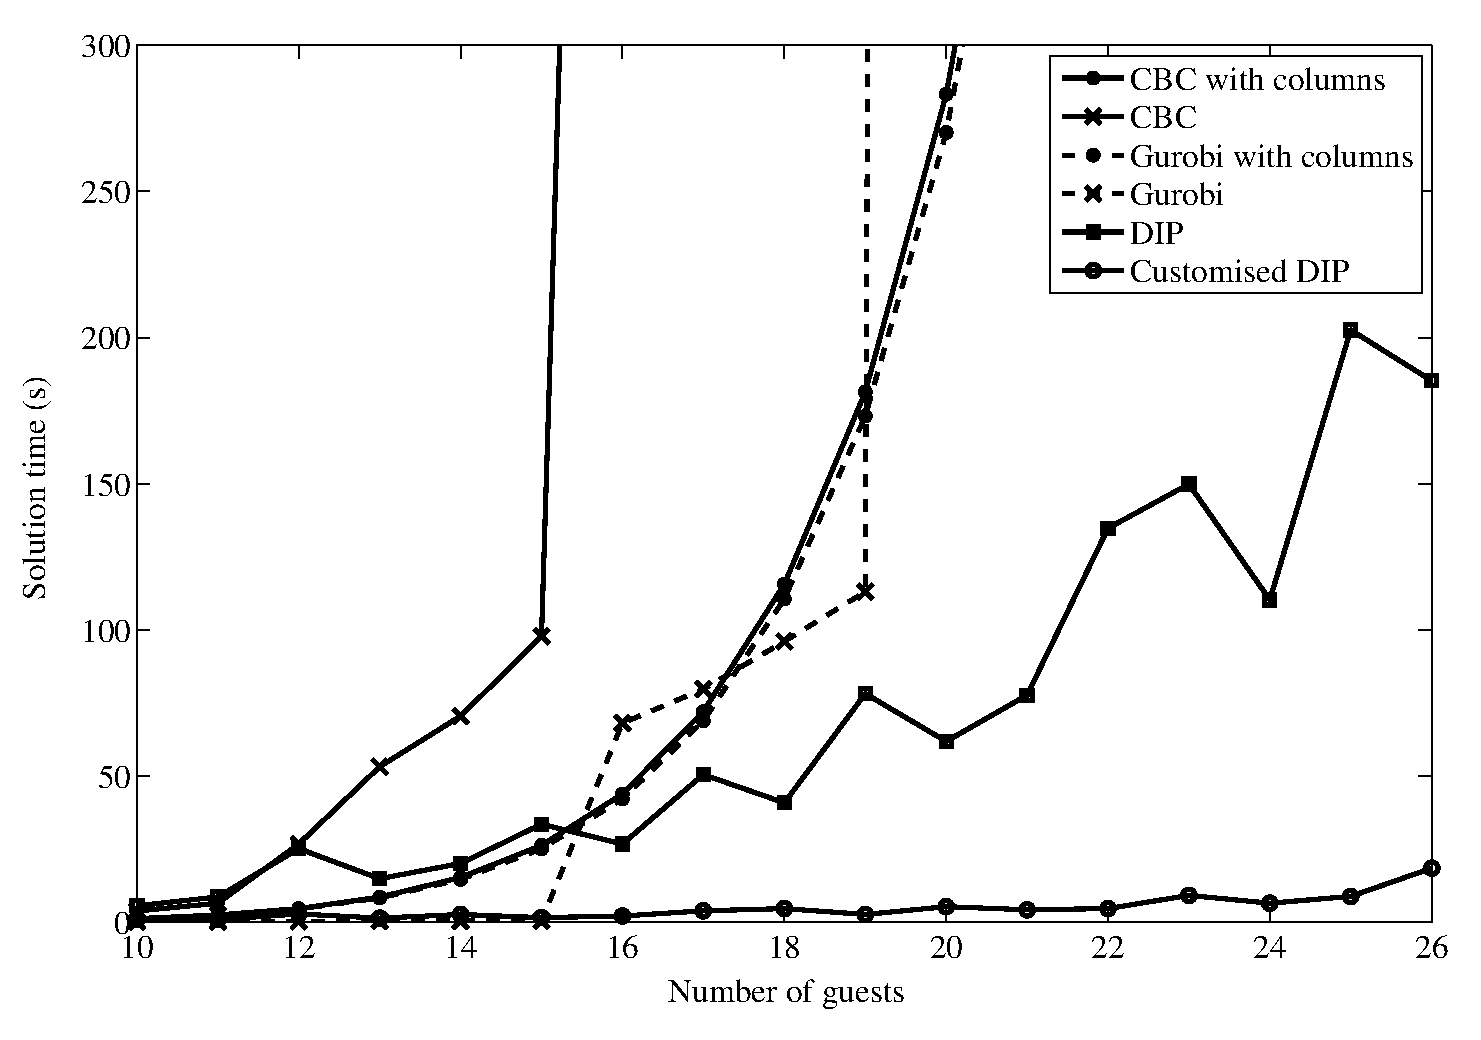
\includegraphics[scale=0.600]{img/wedbench.eps}
\caption{Comparing solver performance on the Wedding Planner problem. 
In this figure the times for generating the columns for ``CBC with columns'' and ``Gurobi with columns'' have been included in the total solve time. The time required for solving the original formulation sharply increases for both Gurobi and CBC (marked with crosses) but at different problem sizes. However the time for the column-wise formulation is similar for Gurobi and CBC. The time for DIP does not smoothly increase with problem size, but is consistently lower than Gurobi for instances with 16 or more guests.} \label{fig:compare}
\end{figure}